\documentclass[12pt]{article}
\usepackage[left=2cm, top=2cm, right=2cm, bottom=2cm]{geometry}
\usepackage[utf8]{inputenc}
\usepackage[T1]{fontenc}
\usepackage[french]{babel}
\usepackage{graphicx}
\usepackage{graphics}
\usepackage{amsmath}
\usepackage{tikz}
\usepackage{graphicx}
\usepackage{xcolor}
\usepackage{parskip}
\usepackage{physics}
\usepackage{gensymb}

\title{\textbf{Instrumentation} \\ TP 2: Caractérisation d'un capteur de température}
\author{MENARD Alexandre \\ VIEILLEDENT Florent \\ RANCHY Nilo}

\setlength{\parindent}{1cm}

\begin{document}
\maketitle

\section*{Introduction}
Dans ce travail pratique, on étudie les caractéristiques d'un capteur de température PT100. Le capteur est composé notamment d'une couche de platine dont la résistance varie en fonction de la température. Le capteur que nous utilisons est de classe B et de type PTFF.100 faisant référence à la résistance $R_0$ du capteur à $0\degree C$. On commence par un circuit d'un pont diviseur de tension. On cherche alors à déterminer la température de la pièce en mesurant la résistance du capteur. On cherche aussi à déterminer le temps de réponse du capteur et on étudie l'influence du courant sur les mesures. On change ensuite le circuit de conditionnement en utilisant un Pont de Wheatstone, pour comparer la sensibilité des deux circuits.

\section{Premier circuit de conditionnement : Pont diviseur de tension}
\subsection{Montage expérimental}
La fiche technique du capteur nous indique un courant recommandé pour nos mesure de $I_{mes}=1.4\, mA$, nous allons donc utiliser un pont diviseur de tension pour avoir le courant recommandé dans notre capteur. Notre montage est composé d'un générateur de tension $E=5.0136\, V$ (mesuré avec un voltmètre), d'une résistance $R=5.085 \, k\Omega$ (mesuré avec un ohmmètre), d'un voltmètre et du capteur de température. On note respectivement $R_{PT}$ et $U_{PT}$ la résistance du capteur et la tension à ses bornes. 

Pour calculer la température de la pièce, on commence par calculer $R_{PT}$ avec un ohmmètre. Puis on calcule $U_{PT}$ avec le circuit 1 de la figure (\ref{Schéma_exp1}).

Pour mesurer le temps de réponse du capteur, on réutilise le même circuit. On commence par chauffer le capteur en le tenant dans nos doigts. Puis on filme le voltmètre avec un chronomètre à côté et on laisse refroidir le capteur. On note toutes les secondes la tension aux bornes du capteur.  

\newpage
\begin{figure}[h!]
	\begin{center}
		\includegraphics[scale=0.1]{Schéma_exp1.png}
		\label{Schéma_exp1}
		\caption{Gauche : Circuit 1 pour mesurer la température de la pièce et calculer le temps de réponse. Droite : Circuit 2 pour déterminer la relation entre l'intensité et la température}
	\end{center}
\end{figure}

On utilise ensuite le circuit 2. On mesure $U_{PT}$ en faisant varier la résistance du potentiomètre $R_{Pot}$ de 3500 à 250 $\Omega$.

\subsection{Modèle}
D'après la fiche technique du capteur, on a la relation suivante pour $T\geq 0\degree C$:
\begin{equation}
R_{PT}=R_0(1+a*T+b*T^2)
\end{equation}
avec $a=3.9083*10^{-3}$ et $b=-5.775*10^{-7}$. Dans notre cas, on utilise une approximation linéaire de cette formule:
\begin{equation}
R_{PT}=R_0(1+a*T)
\label{Modèle_linéaire}
\end{equation}

On calcule la différence entre ces deux modèles. On remarque que pour des températures ambiantes (entre $0$ et $40\degree C$), la différence de température entre les deux modèles est inférieure à $0.25\degree C$. On accepte cet écart pour cette première expérience mais il faudra prendre en compte cette différence dans nos conclusions. 
\begin{figure}[h!]
	\begin{center}
		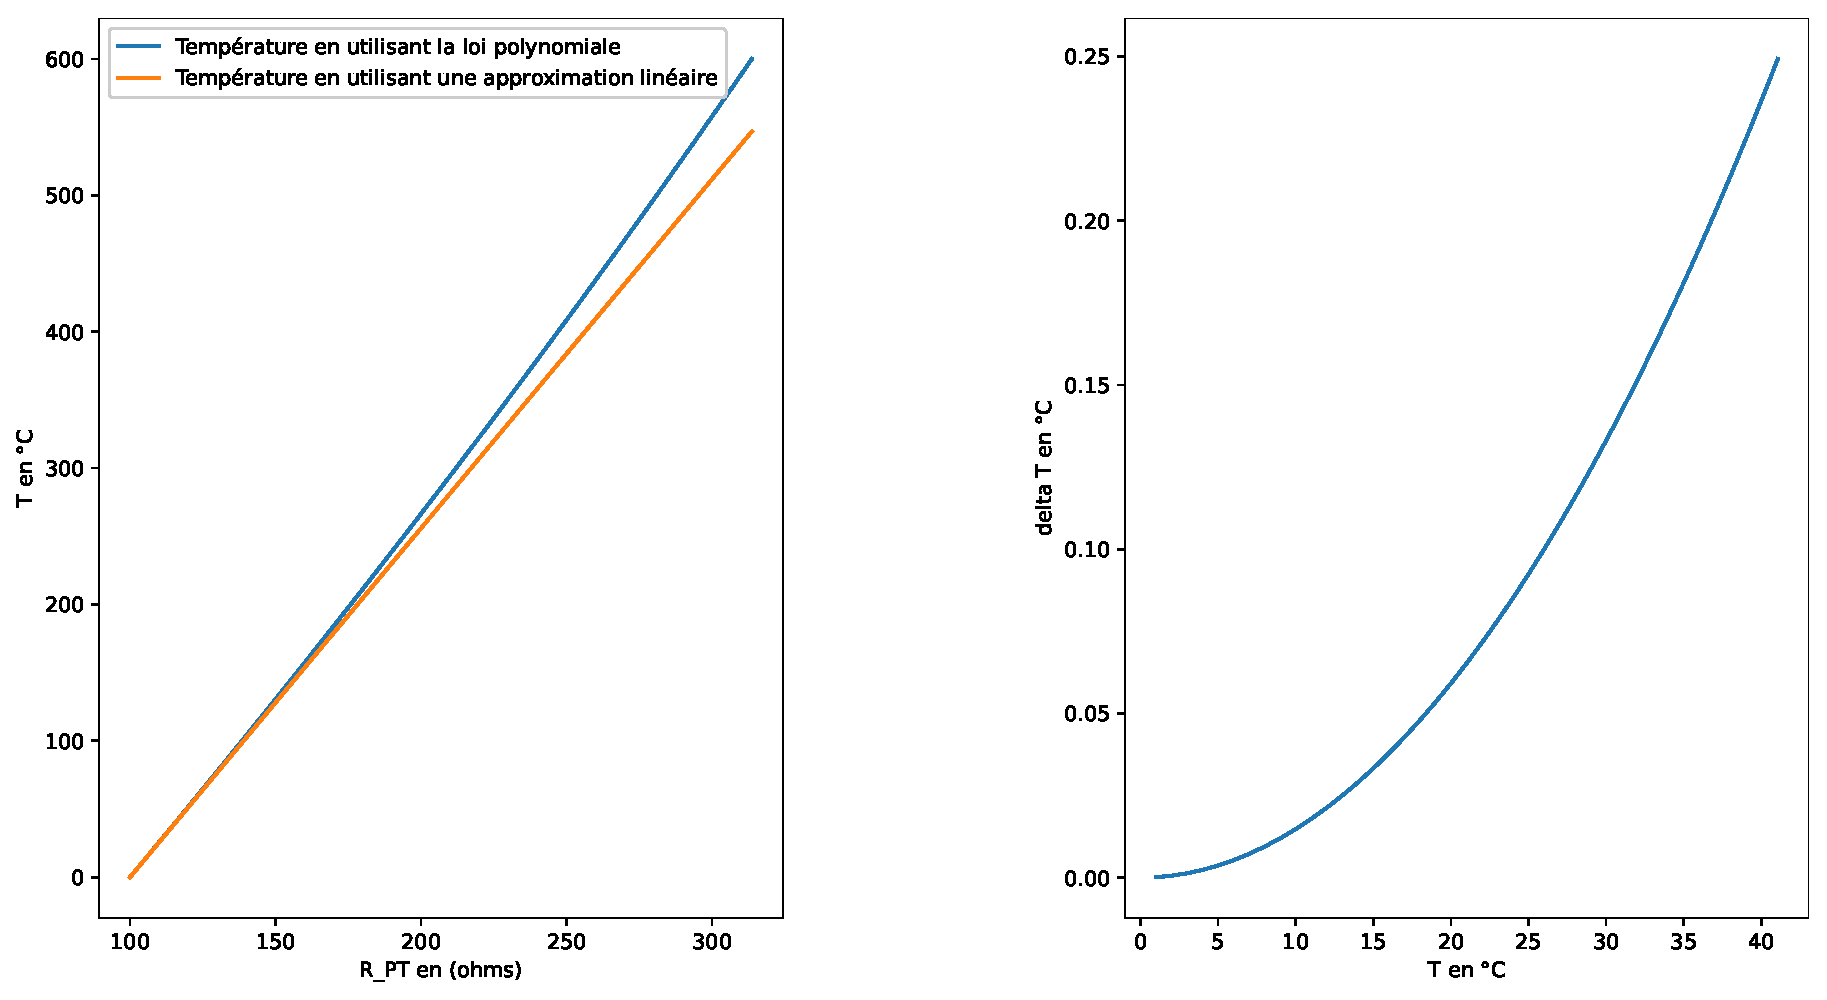
\includegraphics[scale=0.3]{Comparaison.eps}
		\label{Comparaison}
		\caption{Gauche: Comparaison des températures calculées avec les deux modèles. Droite: Différence entre les modèles pour des température ambiantes}
	\end{center}
\end{figure}

D'après l'équation (\ref{Modèle_linéaire}), on a donc la relation suivante:
\begin{equation}
T=\frac{R_{PT}-R_0}{a*R_0}
\label{Equation_température}
\end{equation}

En utilisant la formule du pont diviseur de tension, on trouve la relation entre $R_{PT}$ et $U_{PT}$:
\begin{align}
U_{PT}=\frac{R_{PT}}{R+R_{PT}}E \Rightarrow R_{PT}=\frac{R*U_{PT}}{E-U_{PT}}
\label{Equa_resistance}
\end{align}

Pour calculer l'intensité $i$ qui traverse la capteur : 
\begin{equation}
i=\frac{E}{R+R_{PT}}
\label{Equa_intensité}
\end{equation}

On s'attend à ce que la température suive une loi exponentielle au fil du temps. Si on note $T_A$ la température de la pièce, $T_0$ la température à laquelle on chauffe le capteur et $\tau$ le temps caractéristique du capteur, on a :
\begin{align}
T(t)&=T_A+(T_0-T_A)*e^{-\frac{t}{\tau}}\Rightarrow
(T(t)-T_A)=(T_0-T_A)*e^{-\frac{t}{\tau}}
\label{exponentielle}
\end{align}   

La fiche technique nous donne un $\tau_{0.9}=10\, s$, ce qui correspond à 
\begin{equation}
1-e^{\frac{\tau_{0.9}}{\tau}}=0.9 \Rightarrow \tau_{0.9}=ln(\frac{1}{0.1})*\tau
\label{Equa_tempsréponse}
\end{equation}

Lorsqu'on diminue beaucoup la résistance du potentiomètre, on augmente l'intensité du courant. L'effet Joule va donc augmenter. On rappelle l'expression de l'effet Joule: $P=RI^2$. La fiche technique nous donne un coefficient d'auto-chauffage en $\degree C/mW$, qu'on note $a$. Par analyse dimensionnelle, on a la relation suivante :
\begin{equation}
\delta T=a*P=a*i^2*R_{PT}
\label{Equation_puissance}
\end{equation}



\subsection{Mesures et interprétations}

On commence par mesurer la température de la pièce. On mesure $U_{PT}=105.97\pm 0.02\, mV$. On fait l'application numérique en utilisant l'équation (\ref{Equa_resistance}) et on trouve $R_{PT}=109.80\, \Omega$. On utilise la méthode de la dérivée pour trouver l'incertitude :
\begin{align*}
\delta R_{PT}&=\frac{dR_{PT}}{dU_{PT}}*\delta U_{PT} \\
\delta R_{PT}&=\frac{R*E}{(E-U_{PT})^2}*\delta U_{PT} \\
\delta R_{PT}&=\frac{5.085.10^{3}*5.0136}{(5.0136-105.97*10^{-3})}*(0.02*10^{-3})\\
\delta R_{PT}&=0.02\, \Omega
\end{align*}

On utilise ensuite l'équation (\ref{Equation_température}) et on obtient $T=25.07 \degree C$. On calcule aussi l'incertitude : $\delta T = \frac{\delta R_{PT}}{a*R_0}=0.05 \degree C$. On a donc $T=25.07\pm 0.05 \degree C$. On a aussi mesuré le température avec un thermocouple et on obtient $T_{thermocouple}=25.0\pm 0.5 \degree C$. Les valeurs sont cohérentes. 
En effectuant une mesure directe de la résistance du capteur avec un ohmmètre, on trouve une résistance $R_{PT}=108.19\pm 0.01 \, \Omega$. Néanmoins, l'ohmmètre ne permet pas de réaliser des circuits de conditionnement, ce qui limite la précision sur la valeur finale de la température, car on ne peut pas améliorer la résolution sur l'ohmmètre. 

On cherche maintenant à déterminer le temps de réponse. On regroupe les données de tension en fonction du temps dans un tableau, donné en annexe.


Grâce aux équations (\ref{Equa_resistance}) et (\ref{Equation_température}), on calcule la température associée à chaque tension. On trace $\Delta T=T-T_A$ en fonction du temps, avec $T_A$ la dernière température mesurée.

\begin{figure}[h!]
	\begin{center}
		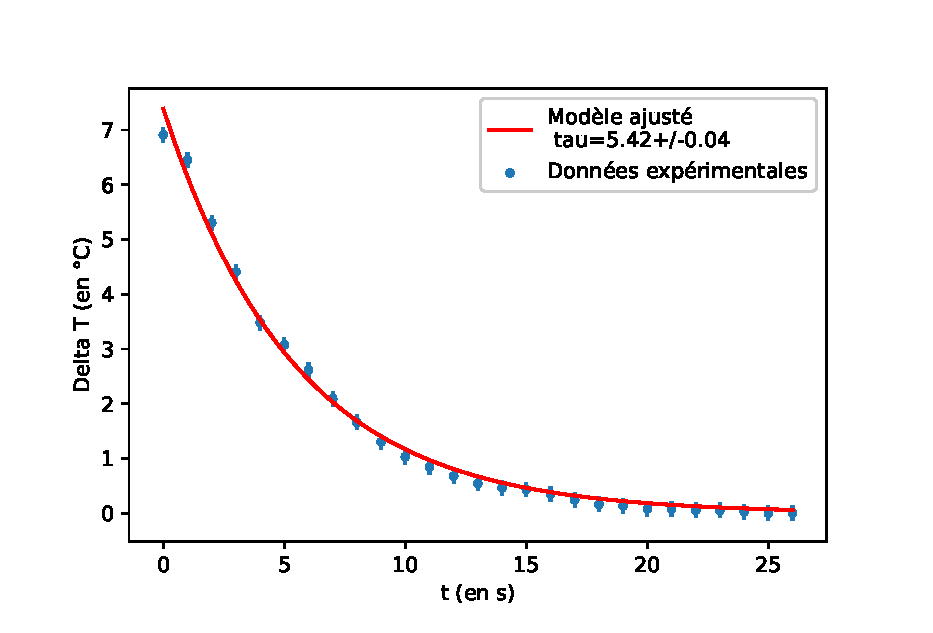
\includegraphics[scale=0.7]{Tempscara.eps}
		\caption{$\Delta T$ en fonction du temps et courbe ajustée}
		\label{Temps_caractéristique}
	\end{center}
\end{figure}

On trouve bien une courbe exponentielle, il y a donc un accord qualitatif avec l'équation (\ref{exponentielle}). On ajuste la courbe avec Python et on trouve un $\tau = 5.42\pm 0.04\,s$. Grâce à l'équation (\ref{Equa_tempsréponse}), on calcule notre temps de réponse expérimentale $\tau_{0.9}=12.48\pm 0.09\,s$.

La documentation nous fournit un $\tau_{0.9} = 10s$ pour une vitesse de l'air $v = 1m/s$. On note donc un écart avec la valeur théorique annoncée de $2.48s$, mais cette différence peut s'expliquer en partie par 
une vitesse de l'air différente lors de notre expérience, que l'on ne contrôle pas, et que l'on ne peut pas mesurer. 

On étudie maintenant l'influence du courant sur nos mesures. En faisant varier $R_{pot}$, on obtient les données du deuxième tableau en annexe.


On calcule donc $i$ l'intensité dans le capteur grâce à l'équation (\ref{Equa_intensité}), puis la température grâce aux équations (\ref{Equa_resistance}) et (\ref{Equation_température}). On trace $\Delta T=T-T_A$ en fonction de l'intensité, avec $T_A$ la température de la pièce. Pour mieux visualiser, on trace ensuite $\Delta T$ en fonction de la puissance. D'après l'équation ($\ref{Equation_puissance}$), on est censé obtenir une droite. On remarque dans les deux graphiques de la figure (\ref{Graphe_puissance}) que les premiers points semblent aberrants. Les autres points du deuxième graphique semblent néanmoins tracer une droite, on peut dire qu'il y a un accord qualitatif.
\begin{figure}[h!]
	\begin{center}
		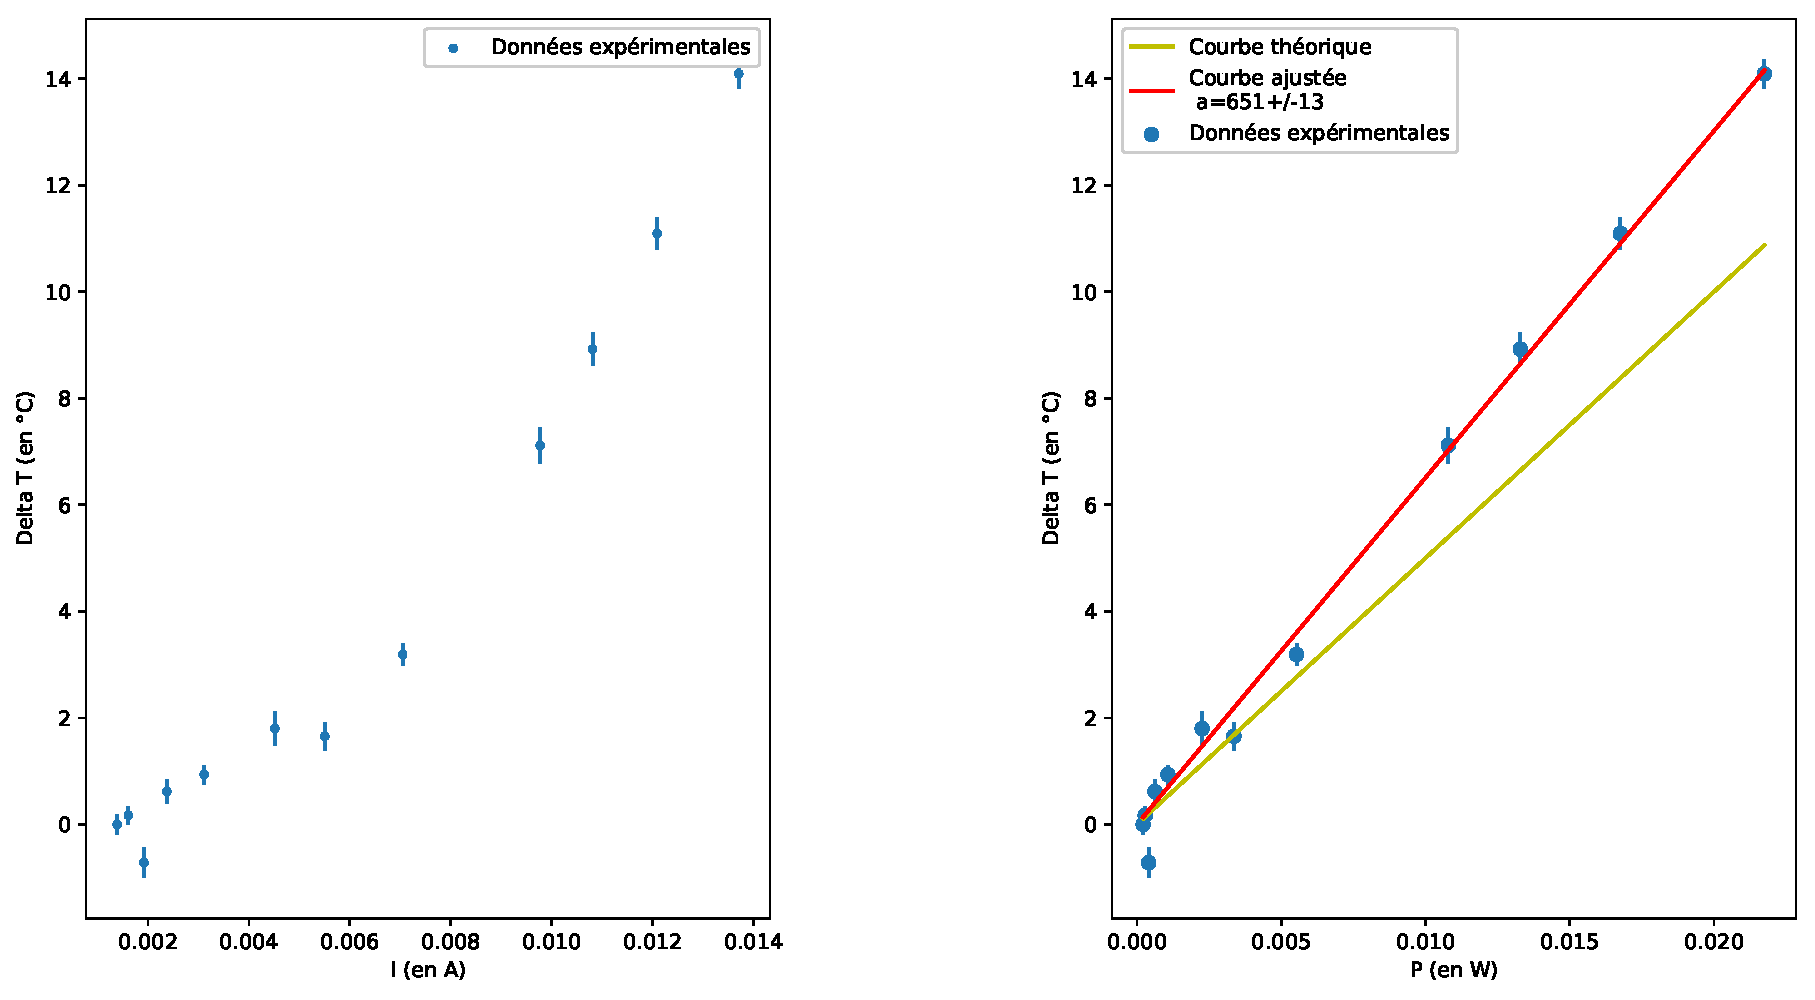
\includegraphics[scale=0.5]{Graphe2_puissance.eps}		
		\caption{Gauche: Graphique de $\Delta T$ en fonction du courant dans la capteur. Droite: Graphique de la température générée par effet Joule en fonction de la puissance}
		\label{Graphe_puissance}
	\end{center}
\end{figure}

 On fait donc une régression linéaire et on obtient  un coefficient linéaire $a=651\pm 13\, \degree C/W$. La valeur théorique donné par la fiche technique est de $500\, \degree C/W$. Il n'y a pas d'accord quantitatif, l'écart relatif est de $30\%$. Cet écart peut en partie s'expliquer car la valeur théorique est donné pour un mouvement d'air de $1\, m/S$, ce qui n'est sûrement pas le cas dans notre montage.
 
Néanmoins, l'écart est important et nous avons des points aberrants, il faudrait donc refaire l'expérience, notamment en mesurant directement l'intensité dans notre circuit. 

\section{Deuxième circuit de conditionnement : Pont de Wheatstone}
\subsection{Montage expérimental}

On réalise un pont de Wheatstone avec une résistance $R'$ de $2\, k\Omega$, 2 résistances $R$ de $200\,\Omega$, un potentiomètre $R_{pot}$ réglé sur $110\, \Omega$, un générateur de tension de $5.0136\, V$, un voltmètre et notre capteur de température. On s'assure de ne jamais placer B ou D à la masse, pour que le courant ne passe pas que dans une branche de notre circuit.

\begin{figure}[h!]
	\begin{center}
		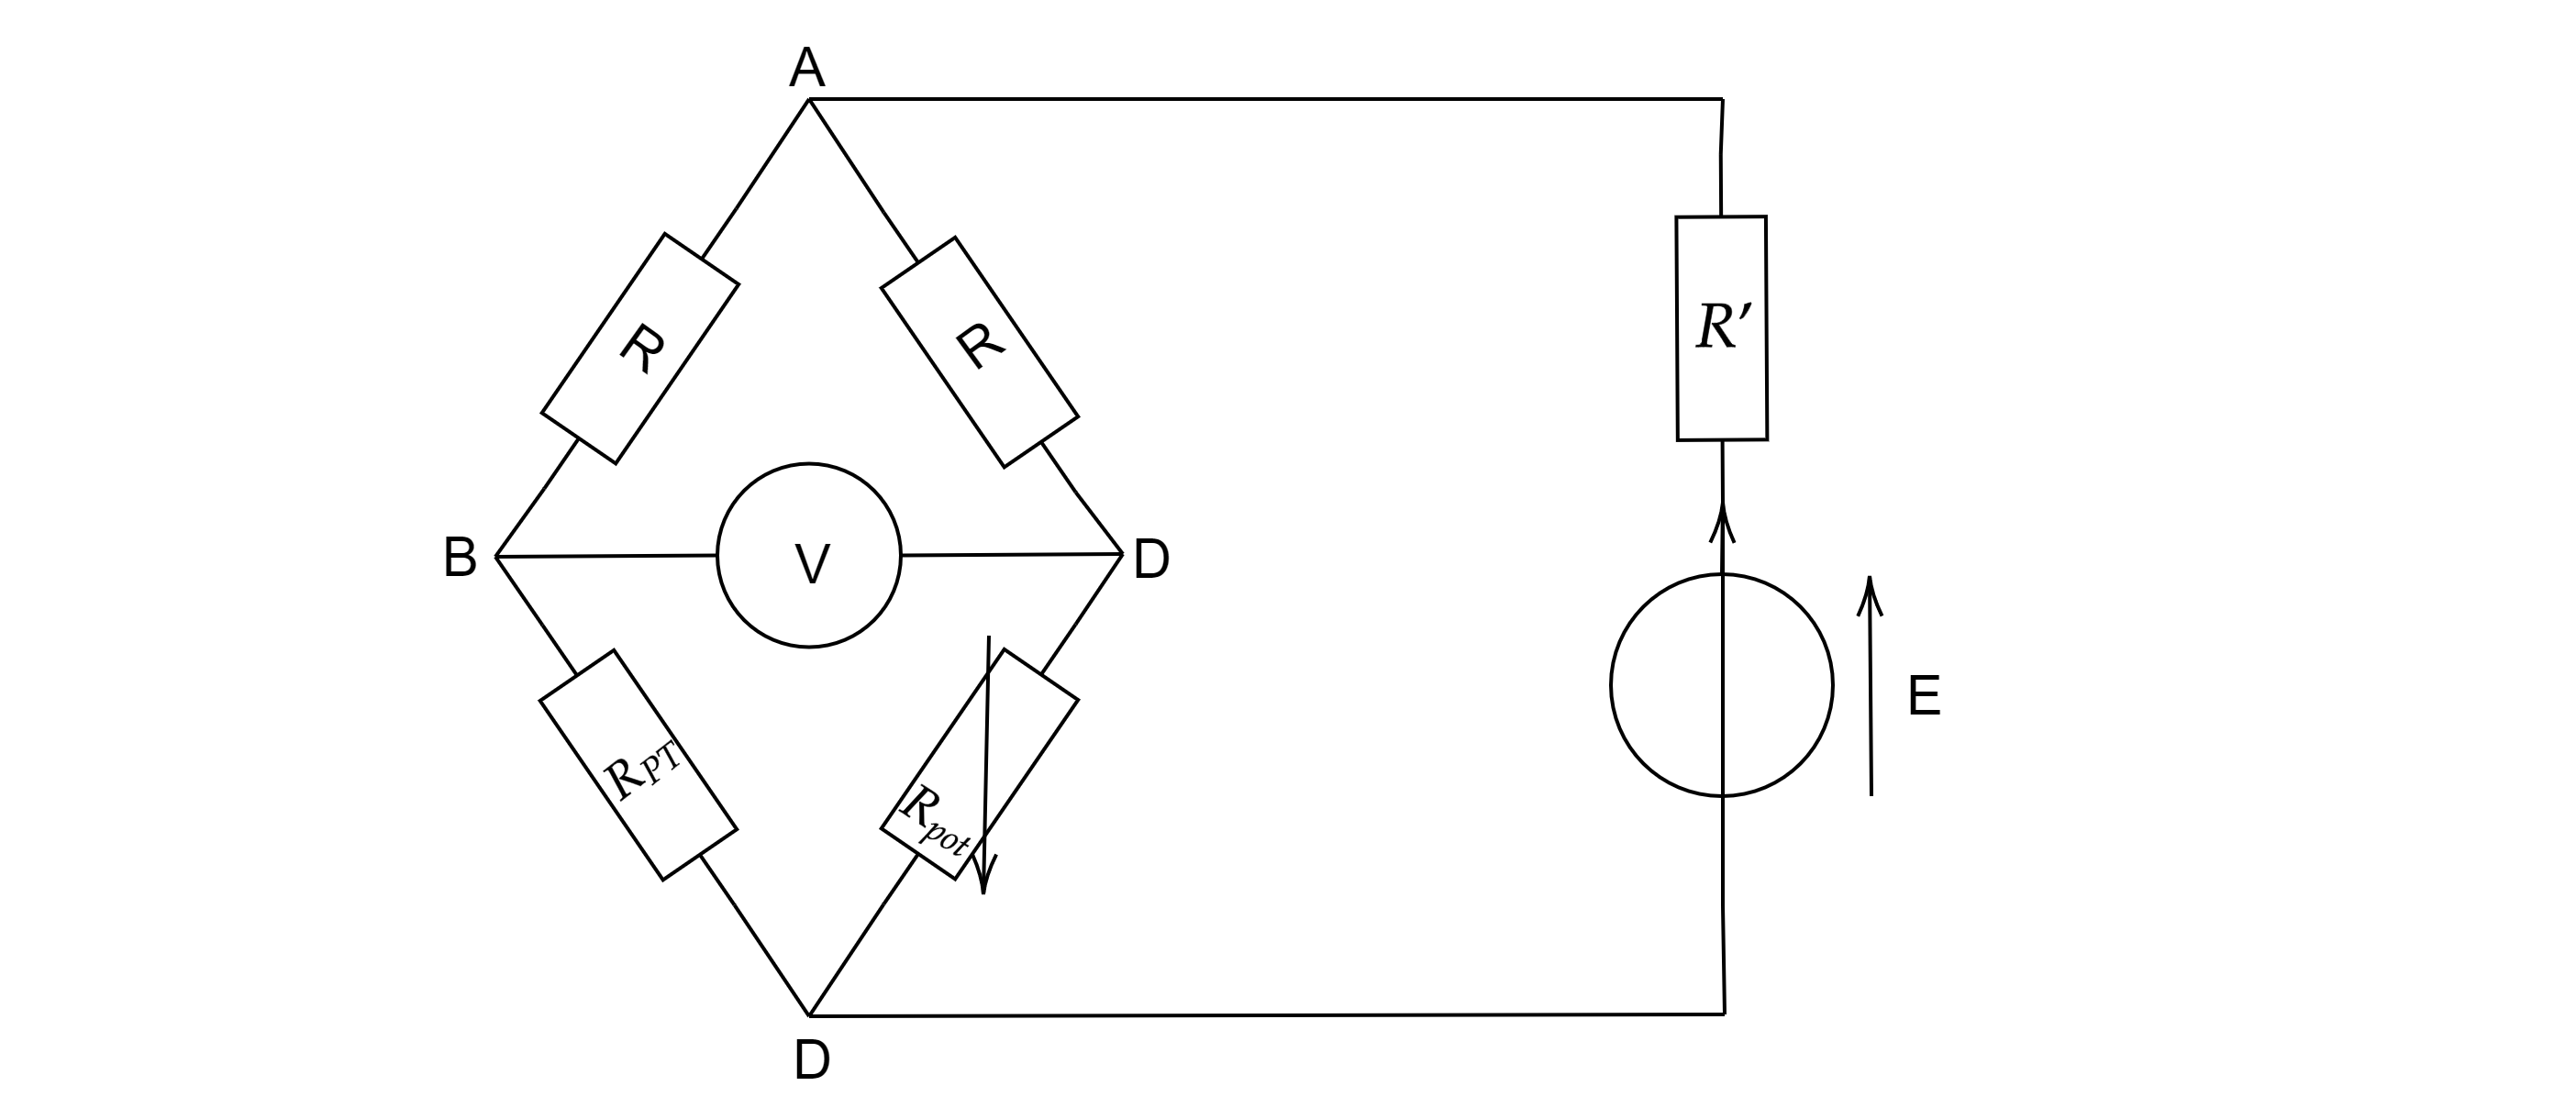
\includegraphics[scale=0.1]{Wheatstone.png}
		\caption{Circuit du pont de Wheastone}
		\label{Wheatstone}
	\end{center}
\end{figure}

\subsection{Modèle}

On détermine l'intensité $i$ qui traverse notre capteur en utilisant des résistances équivalentes et l'équivalence Thévenin/Norton :
\begin{equation}
i=\frac{\frac{R'*(R_{pot}+R)}{R'+(R_{pot}+R)}}{\frac{R'*(R_{pot}+R)}{R'+(R_{pot}+R)}+(R+R_{PT})}*\frac{E}{R'}
\label{Intensité_wheatstone}
\end{equation}

La tension $U_{BD}$ est trouvé en calculant $V_B - V_D$, est deux potentiel étant égal respectivement à $V_{BC}$ et $V_{DC}$, qu'on trouve en utilisant la formule du pont diviseur de tension. Finalement on obtient:
\begin{equation}
U_{BD}=(\frac{R_{PT}}{R_{PT}+R}-\frac{R_{pot}}{R+R_{pot}})*E
\label{Tension_wheatstone}
\end{equation}

On obtient:
\begin{equation}
R_{PT}=\frac{R(\frac{U_{BD}}{E}+\frac{R_{pot}}{R_{pot}+R})}{1-\frac{U_{BD}}{E}+\frac{R_{pot}}{R_{pot}+R}}
\label{Resistance_wheatstone}
\end{equation}

On remarque que pour que $U_{BD}=0$, il faut que $R_{pot}=R_{PT}$.

\subsection{Mesures et interprétations}

On commence par vouloir mesurer le courant qui traverse notre capteur. Pour cela on mesure $U_{AC}=362.4\, mV$ et on utilise la loi d'ohm et la loi des nœuds, avec $I_0$ l'intensité dans la branche du générateur et $i_2$ l'intensité dans la branche du potentiomètre :
\begin{equation}
i=I_0-i_2=\frac{E}{R'}-\frac{U_{AC}}{R+R_{pot}}=1.33\, mA
\end{equation}
On a bien un courant proche de $I_{mes}$.

On mesure une tension $U_{BD}=-0.20\pm 0.01\, mV$. En faisant l'application de l'équation (\ref{Resistance_wheatstone}), on obtient $R_{PT}=109.981\pm 0.004\, \Omega$. On trouve une valeur cohérente avec le premier circuit de conditionnement. Néanmoins, le pont de Wheatstone permet de mesurer uniquement la variation de la tension aux bornes du capteur. Le premier circuit de conditionnement mesurait directement la valeur de cette tension, qui peut être beaucoup plus grande que sa variation, et donc gêner la mesure en augmentant la résolution du capteur. La résolution et donc la précision de notre mesure est donc améliorée avec le deuxième circuit. 

\newpage

\section*{Conclusion}
Dans ce travail pratique, on a étudié un capteur de température PT100. On a commencé par déterminer la température de la pièce en mesurant la résistance du capteur. Pour cela, on a mesuré la tension aux bornes du capteur en utilisant un pont diviseur de tension. En utilisant une relation linéaire entre la résistance du capteur et la température, on a pu déterminer la température de la pièce. On a trouvé un résultat en accord avec la valeur donnée par un thermocouple. Un moyen d'améliorer notre expérience serait d'utiliser le modèle complet (pas linéaire). 

On a ensuite mesuré le temps de réponse du capteur. Pour cela on a commencé par le chauffer, puis on l'a laissé refroidir en mesurant la température au fil du temps. On trouve un temps de réponse d'environ 12.5 secondes, alors que la valeur théorique est de 10 secondes. On a expliqué cet écart par le fait que la valeur théorique est donnée pour un mouvement d'air de 1 mètre par seconde, ce qui n'était pas le cas dans notre expérience. Il faudrait donc refaire l'expérience en contrôlant la vitesse de l'air, par exemple avec un ventilateur.

On a de plus étudié l'effet du courant sur nos mesures. On a remarqué quand augmentant l'intensité, le capteur commençait à chauffer à cause de l'effet Joule. On a établi une relation linéaire entre la puissance du capteur et sa température. Le coefficient qu'on a obtenu n'était pas le même fournit par la documentation. On attribue encore cela au mouvement d'air. Il faudrait là encore refaire l'expérience en contrôlant ce paramètre. 

On a ensuite changé notre circuit de conditionnement pour utiliser un pont de Wheatstone. On a remarqué que la résolution était meilleure lorsqu'on utilisait ce circuit.  



\newpage


\section*{Annexes}
\begin{table}[!h]
	\begin{small}
	\begin{center}
		\begin{tabular}{|c|c|}
\hline
 t $\pm 0.1$ (en s) &  $U_{PT}\pm 0.05$ (en mV) \\
\hline

       0 &        110.58 \\
        1 &        110.41 \\
        2 &        109.99 \\
        3 &        109.66 \\
        4 &        109.32 \\
        5 &        109.17 \\
        6 &        109.00 \\
        7 &        108.81 \\
        8 &        108.65 \\
        9 &        108.52 \\
       10 &        108.42 \\
       11 &        108.35 \\
       12 &        108.29 \\
       13 &        108.24 \\
       14 &        108.21 \\
       15 &        108.20 \\
       16 &        108.17 \\
       17 &        108.13 \\
       18 &        108.10 \\
       19 &        108.09 \\
       20 &        108.07 \\
       21 &        108.07 \\
       22 &        108.06 \\
       23 &        108.06 \\
       24 &        108.05 \\
       25 &        108.04 \\
       26 &        108.04 \\

\hline
	\end{tabular}
	\end{center} \end{small}
	\label{Tableau_Data}
	\caption{Données pour calculer le temps de réponse}
\end{table}


\begin{table}[h!]
	\begin{center}
		\begin{tabular}{|c|c|}
\hline
 $R_{pot}\pm 1$ (en\,$ \Omega$) &  U (en mV) \\
\hline
  $3500$ &      $153.0\pm 0.5$ \\
  $3000$ &      $177.7\pm 0.5$ \\
  $2500$ &      $211.1\pm 0.5$ \\
  $2000$ &      $262.3\pm 0.5$ \\
  $1500$ &      $344.1\pm 0.5$ \\
  $1000$ &      $500.4\pm 0.5$ \\
   $800$ &      $610.0\pm 0.5$ \\
   $600$ &      $785.2\pm 0.5$ \\
   $400$ &     $1104 \pm 1$ \\
   $350$ &     $1229 \pm 1$ \\
   $300$ &     $1385 \pm 1$ \\
   $250$ &     $1586\pm 1$ \\
\hline
\end{tabular}
	\end{center}
	\label{Tableau_puissance}
	\caption{Valeurs de la tension aux bornes du capteur pour différentes valeurs de résistance du potentiomètre}
\end{table}


\end{document}
